\chapter{Sortieralgorithmen}
\begin{center}  
\begin{tabular}{|p{3.2cm}|c|c|c|c|}
    \hline
    Sortieralgorithmus & Best-Case &
    Worst-Case & Average-Case &
    Stabil \\
    \hline
    Bubblesort & $O(n)$ & $O(n^2)$ & $O(n^2)$ & Ja \\
    \hline
    Insertionsort & $O(n)$ & $O(n^2)$ & $O(n^2)$ & Ja \\
    \hline
    Selectionsort & $O(n^2)$ & $O(n^2)$ & $O(n^2)$ & Nein \\
    \hline
    Quicksort & $O(n\log n)$ & $O(n^2)$ & $O(n\log n)$ & Nein \\
    \hline
\end{tabular}
\end{center}

\begin{center}
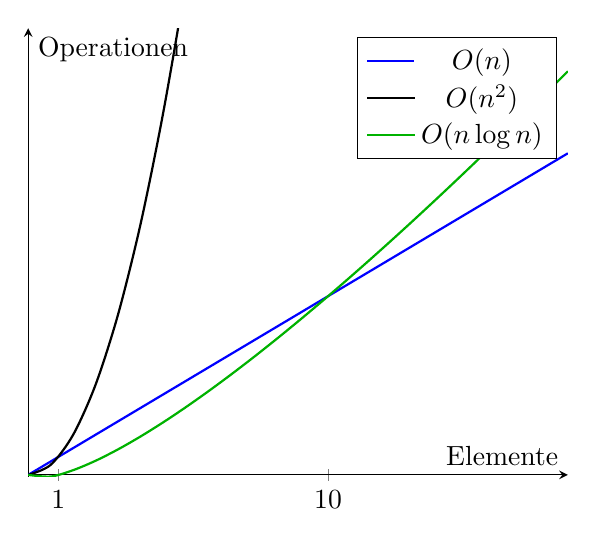
\begin{tikzpicture}
\begin{axis}[axis lines=middle,
             domain=0:18,ymax=25,
             xtick={1,10},ytick={0},
             xlabel={Elemente},
             ylabel={Operationen}]
    \addplot[blue,thick] {x};
    \addlegendentry{$O(n)$}
    \addplot[black,thick,smooth] {x^2};
    \addlegendentry{$O(n^2)$}
    \addplot[black!30!green,thick,smooth] {x*log10(x)};
    \addlegendentry{$O(n\log n)$}
\end{axis}
\end{tikzpicture}
\end{center}

\section{Bubblesort}
\begin{center}  
\begin{tabular}{c|c|c}
1. Durchlauf & 2. Durchlauf & 3. Durchlauf \\
\begin{tikzpicture}
    \matrix (A) [matrix of nodes,row sep=2cm,nodes={draw, minimum size=8mm},column sep=-\pgflinewidth]{
        3 & 4 & 2 & 1 \\
        3 & 4 & 2 & 1 \\
        3 & 2 & 4 & 1 \\
    };
    \path[->]
        (A-2-2) edge [bend left=90] node [above] {$4>2$} (A-2-3)
        (A-3-3) edge [bend left=90] node [above] {$4>1$} (A-3-4);
    \path
        (A-1-1) node [below=12pt] {$i$}
        (A-1-2) node [below=12pt] {$j$}
        (A-2-2) node [below=12pt] {$i$}
        (A-2-3) node [below=12pt] {$j$}
        (A-3-3) node [below=12pt] {$i$}
        (A-3-4) node [below=12pt] {$j$};
\end{tikzpicture}
&
\begin{tikzpicture}
    \matrix (A) [matrix of nodes,row sep=2cm,nodes={draw, minimum size=8mm},column sep=-\pgflinewidth]{
        3 & 2 & 1 & 4 \\
        2 & 3 & 1 & 4 \\
        2 & 3 & 1 & 4 \\
    };
    \path[->]
        (A-1-1) edge [bend left=90] node [above] {$3>2$} (A-1-2)
        (A-2-2) edge [bend left=90] node [above] {$3>1$} (A-2-3);
    \path
        (A-1-1) node [below=12pt] {$i$}
        (A-1-2) node [below=12pt] {$j$}
        (A-2-2) node [below=12pt] {$i$}
        (A-2-3) node [below=12pt] {$j$}
        (A-3-3) node [below=12pt] {$i$}
        (A-3-4) node [below=12pt] {$j$};
\end{tikzpicture}
&
\begin{tikzpicture}
    \matrix (A) [matrix of nodes,row sep=2cm,nodes={draw, minimum size=8mm},column sep=-\pgflinewidth]{
        2 & 1 & 3 & 4 \\
        1 & 2 & 3 & 4 \\
        \\
    };
    \path[->]
        (A-1-1) edge [bend left=90] node [above] {$2>1$} (A-1-2);
    \path
        (A-1-1) node [below=12pt] {$i$}
        (A-1-2) node [below=12pt] {$j$};
\end{tikzpicture}
\end{tabular}
\end{center}

\begin{center}  
\begin{lstlisting}
// BubbleSort.java

// Wird fuer Arrays.toString() benoetigt
import java.util.Arrays;

public class BubbleSort {
    public static void main(String[] args) {
        int[] ints = {3,4,2,1};
        for (int i = 0; i < ints.length; i++) {
            for (int j = i+1; j < ints.length; j++) {
                if (ints[j] < ints[i]) {
                    int tmp = ints[j];
                    ints[j] = ints[i];
                    ints[i] = tmp;
                }
            }
        }
        System.out.println(Arrays.toString(ints));
    }
}
\end{lstlisting}
\end{center}

\section{Insertionsort}
\begin{center}
\begin{tabular}{r|l}
sortiert & unsortiert \\
&
\begin{tikzpicture}
    \matrix (A) [matrix of nodes,
                 row sep=2cm,
                 nodes={draw, minimum size=8mm},
                 column sep=-\pgflinewidth] {
        3 & 4 & 2 & 1 \\
    };
\end{tikzpicture} \\
\begin{tikzpicture}
    \matrix (A) [matrix of nodes,
                 row sep=2cm,
                 nodes={draw, minimum size=8mm},
                 column sep=-\pgflinewidth] {
        3 \\
    };
\end{tikzpicture} &
\begin{tikzpicture}
    \matrix (A) [matrix of nodes,
                 row sep=2cm,
                 nodes={draw, minimum size=8mm},
                 column sep=-\pgflinewidth,
                 column 1/.style={nodes={fill=teal!25}}]{
        4 & 2 & 1 \\
    };
\end{tikzpicture} \\
\begin{tikzpicture}
    \matrix (A) [matrix of nodes,
                 row sep=2cm,
                 nodes={draw, minimum size=8mm},
                 column sep=-\pgflinewidth,
                 column 2/.style={nodes={fill=teal!25}}]{
        3 & 4\\
    };
\end{tikzpicture} &
\begin{tikzpicture}
    \matrix (A) [matrix of nodes,
                 row sep=2cm,
                 nodes={draw, minimum size=8mm},
                 column sep=-\pgflinewidth,
                 column 1/.style={nodes={fill=magenta!25}}]{
        2 & 1 \\
    };
\end{tikzpicture} \\
\begin{tikzpicture}
    \matrix (A) [matrix of nodes,
                 row sep=2cm,
                 nodes={draw, minimum size=8mm},
                 column sep=-\pgflinewidth,
                 column 1/.style={nodes={fill=magenta!25}}]{
        2 & 3 & 4\\
    };
\end{tikzpicture} &
\begin{tikzpicture}
    \matrix (A) [matrix of nodes,
                 row sep=2cm,
                 nodes={draw, minimum size=8mm},
                 column sep=-\pgflinewidth,
                 column 1/.style={nodes={fill=cyan!25}}]{
        1 \\
    };
\end{tikzpicture} \\
\begin{tikzpicture}
    \matrix (A) [matrix of nodes,
                 row sep=2cm,
                 nodes={draw, minimum size=8mm},
                 column sep=-\pgflinewidth,
                 column 1/.style={nodes={fill=cyan!25}}]{
        1 & 2 & 3 & 4\\
    };
\end{tikzpicture} & \\
\end{tabular}
\end{center}

\begin{center}
\begin{lstlisting}
// InsertionSort.java

// Wird fuer Arrays.toString() benoetigt
import java.util.Arrays;

public class InsertionSort {
    public static void main(String[] args) {
        int[] ints = {3,4,2,1};
        for (int i = 1; i < ints.length; i++) {
            int key = ints[i];
            int j = i-1;
            while (j >= 0 && ints[j] > key) {
                ints[j+1] = ints[j];
                j--;
            }
            ints[j+1] = key;
        }
        System.out.println(Arrays.toString(ints));
    }
}
\end{lstlisting}
\end{center}

\section{Selectionsort}
\begin{center}
\begin{tabular}{r|l}
sortiert & unsortiert \\
&
\begin{tikzpicture}
    \matrix (A) [matrix of nodes,
                 row sep=2cm,
                 nodes={draw, minimum size=8mm},
                 column sep=-\pgflinewidth,
                 column 4/.style={nodes={fill=cyan!25}}] {
        3 & 4 & 2 & 1 \\
    };
\end{tikzpicture} \\
\begin{tikzpicture}
    \matrix (A) [matrix of nodes,
                 row sep=2cm,
                 nodes={draw, minimum size=8mm},
                 column sep=-\pgflinewidth,
                 column 1/.style={nodes={fill=cyan!25}}] {
        1 \\
    };
\end{tikzpicture} &
\begin{tikzpicture}
    \matrix (A) [matrix of nodes,
                 row sep=2cm,
                 nodes={draw, minimum size=8mm},
                 column sep=-\pgflinewidth,
                 column 2/.style={nodes={fill=teal!25}}] {
        4 & 2 & 3 \\
    };
\end{tikzpicture} \\
\begin{tikzpicture}
    \matrix (A) [matrix of nodes,
                 row sep=2cm,
                 nodes={draw, minimum size=8mm},
                 column sep=-\pgflinewidth,
                 column 2/.style={nodes={fill=teal!25}}] {
        1 & 2 \\
    };
\end{tikzpicture} &
\begin{tikzpicture}
    \matrix (A) [matrix of nodes,
                 row sep=2cm,
                 nodes={draw, minimum size=8mm},
                 column sep=-\pgflinewidth,
                 column 2/.style={nodes={fill=magenta!25}}] {
        4 & 3 \\
    };
\end{tikzpicture} \\
\begin{tikzpicture}
    \matrix (A) [matrix of nodes,
                 row sep=2cm,
                 nodes={draw, minimum size=8mm},
                 column sep=-\pgflinewidth,
                 column 3/.style={nodes={fill=magenta!25}}] {
        1 & 2 & 3 \\
    };
\end{tikzpicture} &
\begin{tikzpicture}
    \matrix (A) [matrix of nodes,
                 row sep=2cm,
                 nodes={draw, minimum size=8mm},
                 column sep=-\pgflinewidth] {
        4 \\
    };
\end{tikzpicture} \\
\begin{tikzpicture}
    \matrix (A) [matrix of nodes,
                 row sep=2cm,
                 nodes={draw, minimum size=8mm},
                 column sep=-\pgflinewidth] {
        1 & 2 & 3 & 4\\
    };
\end{tikzpicture} & \\
\end{tabular}
\end{center}

\begin{center}
\begin{lstlisting}
// SelectionSort.java

// Wird fuer Arrays.toString() benoetigt
import java.util.Arrays;

public class SelectionSort {
    public static void main(String[] args) {
        int[] ints = {3,4,2,1};
        for (int i = 0; i < ints.length; i++) {
            int min = i;
            for (int j = i+1; j < ints.length; j++) {
                if (ints[j] < ints[min]) {
                    min = j;
                }
            }
            int tmp = ints[i];
            ints[i] = ints[min];
            ints[min] = tmp;
        }
        System.out.println(Arrays.toString(ints));
    }
}
\end{lstlisting}
\end{center}

\section{Quicksort}
\begin{center}
\begin{tikzpicture}
    \matrix (A) [matrix of nodes,
                 row sep=2cm,
                 nodes={draw, minimum size=8mm},
                 column sep=-\pgflinewidth,
                 column 5/.style={nodes={fill=cyan!25}}] {
        4 & 3 & 1 & 5 & 2 \\
    };
\end{tikzpicture}

\begin{tabular}{c c c}
$<p$ & Pivot $p$ & $>p$ \\
\begin{tikzpicture}
    \matrix (A) [matrix of nodes,
                 row sep=2cm,
                 nodes={draw, minimum size=8mm},
                 column sep=-\pgflinewidth] {
        1 \\
    };
\end{tikzpicture} &
\begin{tikzpicture}
    \matrix (A) [matrix of nodes,
                 row sep=2cm,
                 nodes={draw, minimum size=8mm},
                 column sep=-\pgflinewidth,
                 column 1/.style={nodes={fill=cyan!25}}] {
        2 \\
    };
\end{tikzpicture} &
\begin{tikzpicture}
    \matrix (A) [matrix of nodes,
                 row sep=2cm,
                 nodes={draw, minimum size=8mm},
                 column sep=-\pgflinewidth,
                 column 3/.style={nodes={fill=magenta!25}}] {
        4 & 3 & 5 \\
    };
\end{tikzpicture} \\
& & \begin{tabular}{c c}
\begin{tikzpicture}
    \matrix (A) [matrix of nodes,
                 row sep=2cm,
                 nodes={draw, minimum size=8mm},
                 column sep=-\pgflinewidth,
                 column 2/.style={nodes={fill=teal!25}}] {
        4 & 3 \\
    };
\end{tikzpicture} &
\begin{tikzpicture}
    \matrix (A) [matrix of nodes,
                 row sep=2cm,
                 nodes={draw, minimum size=8mm},
                 column sep=-\pgflinewidth,
                 column 1/.style={nodes={fill=magenta!25}}] {
        5 \\
    };
\end{tikzpicture} \\
\begin{tabular}{c c}
\begin{tikzpicture}
    \matrix (A) [matrix of nodes,
                 row sep=2cm,
                 nodes={draw, minimum size=8mm},
                 column sep=-\pgflinewidth,
                 column 1/.style={nodes={fill=teal!25}}] {
        3 \\
    };
\end{tikzpicture} &
\begin{tikzpicture}
    \matrix (A) [matrix of nodes,
                 row sep=2cm,
                 nodes={draw, minimum size=8mm},
                 column sep=-\pgflinewidth] {
        4 \\
    };
\end{tikzpicture}
\end{tabular} &
\end{tabular}
\end{tabular}
\end{center}

\begin{center}
\begin{tikzpicture}
    \matrix (A) [matrix of nodes,
                 row sep=2cm,
                 nodes={draw, minimum size=8mm},
                 column sep=-\pgflinewidth] {
        1 & 2 & 3 & 4 & 5 \\
    };
\end{tikzpicture}
\end{center}

\begin{center}
\begin{lstlisting}
// QuickSort.java

// Wird fuer Arrays.toString() benoetigt
import java.util.Arrays;

public class QuickSort {
    static int partition(int[] arr, int low, int high) {
        int pivot = arr[high];
        int i = low;

        for (int j = low; j < high; j++) {
            if (arr[j] < pivot) {
                swap(arr, i, j);
                i++;
            }
        }

        swap(arr, i, high);  
        return i;
    }

    static void swap(int[] arr, int i, int j) {
        int temp = arr[i];
        arr[i] = arr[j];
        arr[j] = temp;
    }

    static void quickSort(int[] arr, int low, int high) {
        if (low < high) {          
            int pivot = partition(arr, low, high);

            quickSort(arr, low, pivot - 1);
            quickSort(arr, pivot + 1, high);
        }
    }

    public static void main(String[] args) {
        int[] arr = {10, 7, 8, 9, 1, 5};
        int n = arr.length;
      
        quickSort(arr, 0, n - 1);
        System.out.println(Arrays.toString(arr));
    }
}
\end{lstlisting}
\end{center}
